% Slides de defesa — tese curta (PT-PT).
% ~15 minutos. Regra: um slide, uma ideia. O que está no slide é o que se aponta; o resto diz-se.
% O penúltimo frame é a DEMONSTRAÇÃO (gravação da app).

\documentclass[aspectratio=169]{beamer}
\usetheme{Madrid}
\usecolortheme{seahorse}
\usepackage[T1]{fontenc}
\usepackage[portuguese,shorthands=off]{babel}
\usepackage{booktabs}
\usepackage{tikz}
\usetikzlibrary{positioning, arrows.meta, calc, decorations.pathreplacing}
\tikzset{every node/.append style={execute at begin node={\hyphenpenalty=10000\exhyphenpenalty=10000\relax}}}
% As figuras vem da arvore CANONICA. Antes vinham de ../figures (a arvore antiga, de
% onde estes materiais foram movidos) e de ../../thesis, que foi arquivada. Sem isto o
% LaTeX compila em modo rascunho, o numero de paginas nao muda, e o PDF sai SEM AS
% IMAGENS -- que e um defeito que a contagem de paginas esconde.
\graphicspath{{../figures/}}
\usepackage{xcolor}
% A marca: o verde de `app/assets/logo.svg`, e o "G" e o trocadilho inteiro --
% inveSTIGATE + alliGATOR. Uma macro so, para o nome nunca sair escrito de duas
% maneiras diferentes em dois sitios.
\definecolor{marca}{HTML}{0A8F52}
\newcommand{\gator}{Investi\textcolor{marca}{G}ator}
\setbeamertemplate{navigation symbols}{}
\setbeamertemplate{caption}{\raggedright\insertcaption\par}

\title[\gator]{Explicar sem prever}
\titlegraphic{
\includegraphics[height=1.05cm]{logo_lockup.png}}
% A capa é o título da dissertação partido nos dois pontos: a metade evocativa aqui, a
% substantiva no subtítulo. Somadas dão a cadeia exacta que vai na capa e na submissão,
% palavra por palavra. Foi a passagem de 2026-09-06 que fechou a divergência, quando a
% dissertação passou a chamar-se «Explicar sem prever: ...» e deixou de nomear o sistema
% na capa, como nenhuma das quatro aprovadas o faz.
\subtitle{\normalsize Deteção de anomalias e recuperação de precedentes em alertas financeiros verificáveis}
\author[H.\ Santos]{Henrique José da Silva Santos \\
  \footnotesize Orientador: Prof.\ Luís Gomes \quad Coorientador: Rafael Silva}
\institute[ISEP]{MEIA, Instituto Superior de Engenharia do Porto}
\date{\footnotesize Defesa}

\begin{document}

\begin{frame}\titlepage\end{frame}

% ══ 1. O PROBLEMA ═══════════════════════════════════════════════════════════
\begin{frame}{Uma pessoa abre a aplicação, vê isto, e fica com três perguntas}
\begin{center}
\begin{tikzpicture}
  \node[draw, rounded corners=5pt, minimum width=4.2cm, minimum height=1.5cm, fill=black!4] (t) {};
  \node[font=\small\bfseries] at ([yshift=4.5mm]t.center) {NVDA};
  \node[font=\LARGE\bfseries, text=red!65!black] at ([yshift=-3.5mm]t.center) {$-4{,}1\%$};
\end{tikzpicture}
\end{center}
\vspace{1mm}
\begin{enumerate}
  \item[\textbf{1.}] \textbf{Isto é invulgar?}\\
        \footnotesize 4\% numa empresa calma é muito. Noutra, é terça-feira.\\[2mm]
  \item[\textbf{2.}] \textbf{Foi a empresa, ou foi o mercado?}\\
        \footnotesize Se caiu tudo, a história é outra.\\[2mm]
  \item[\textbf{3.}] \textbf{Já aconteceu antes, e o que se seguiu?}\\
        \footnotesize Houve dias parecidos? O que fez o preço depois?
\end{enumerate}
\vspace{2mm}
\begin{center}
\textbf{As aplicações gratuitas correntes não respondem a nenhuma delas.}\\[1mm]
\footnotesize Há produtos recentes que declaram ir além disso. Nenhum mostra os casos
passados, um a um, com o desfecho medido.
\end{center}
\end{frame}

\begin{frame}{O que existe hoje}
\centering
\small
\begin{tabular}{lcccl}
\toprule
& \textbf{invulgar?} & \textbf{empresa ou mercado?} & \textbf{já aconteceu?} & \textbf{custo} \\
\midrule
Aplicação da corretora & --- & --- & --- & incluído \\
Agregador de notícias & --- & --- & --- & grátis \\
\emph{Robo-advisor} & --- & --- & --- & \% da carteira \\
Terminal profissional & \checkmark & \checkmark & \checkmark & milhares/ano \\
Resumo gerado (2025--26) & \multicolumn{3}{c}{\footnotesize \emph{declaram responder; não mostram a evidência}} & grátis \\
\midrule
\textbf{Este trabalho} & \checkmark & \checkmark & \checkmark & \textbf{grátis} \\
\bottomrule
\end{tabular}
\vspace{5mm}

\begin{center}
Dois produtos recentes declaram responder à mesma pergunta. Nenhum declara \textbf{mostrar
a evidência} — os casos passados, um a um, com data e desfecho medido.\\
\textbf{A diferença que reivindico não é de fluência: é de verificabilidade.}
\end{center}
\end{frame}

% ══ 2. O SISTEMA ════════════════════════════════════════════════════════════
\begin{frame}{O que o sistema faz}
\begin{center}
\begin{tikzpicture}[
  font=\small, >={Stealth[length=2.2mm]},
  gat/.style={draw, rounded corners, fill=black!8, align=center, text width=2.9cm, minimum height=0.9cm},
  sis/.style={draw, rounded corners, fill=black!3, align=center, text width=2.4cm, minimum height=1.5cm},
  sa/.style={draw, rounded corners, fill=black!3, align=center, text width=3.4cm, minimum height=1.5cm},
]
  \node[gat] (g1) {movimento invulgar};
  \node[gat, below=6mm of g1] (g2) {notícia relevante};
  \node[sis] (s) at ($(g1)!0.5!(g2) + (3.9,0)$) {\textbf{InvestiGator}};
  \node[sa, right=1.1cm of s] (o) {alerta explicado\\[2pt]
    \scriptsize o quê · porquê\\ \scriptsize fontes · casos passados};
  \draw[->] (g1) -- (s); \draw[->] (g2) -- (s); \draw[->] (s) -- (o);
\end{tikzpicture}
\end{center}
\vspace{4mm}
\begin{center}
\large E há uma coisa que ele \textbf{recusa} fazer.
\end{center}
\end{frame}

\begin{frame}{Não prevê preços}
\begin{center}
\Large
Nunca diz que vai subir.\\[2mm]
Nunca diz para comprar.\\[2mm]
Nunca mostra um alvo de preço.
\end{center}
\vspace{6mm}
\begin{center}
\normalsize
Parece uma limitação. É o contrário:\\
\textbf{é o que torna tudo o resto verificável.}\\[2mm]
\footnotesize Uma afirmação sobre o que já aconteceu confere-se contra o registo.\\
Uma previsão não se confere.
\end{center}
\end{frame}

% ══ 3. AS TRÊS TÉCNICAS ═════════════════════════════════════════════════════
\begin{frame}{Técnica 1: é invulgar?}
Comparar o dia de hoje com \textbf{os 20 dias anteriores da mesma ação}.
\begin{center}
\begin{tikzpicture}[font=\footnotesize]
  \foreach \i in {0,...,19} { \fill[black!18] (\i*0.28,0) rectangle (\i*0.28+0.2,0.45); }
  \fill[orange!70] (20*0.28,0) rectangle (20*0.28+0.2,1.0);
  \draw[decorate, decoration={brace, amplitude=4pt}, black!55] (0,-0.12) -- (19*0.28+0.2,-0.12)
    node[midway, below=5pt, black!65] {os 20 dias anteriores};
  \draw[decorate, decoration={brace, amplitude=4pt}, orange!75!black]
    (20*0.28,-0.12) -- (20*0.28+0.2,-0.12) node[midway, below=5pt, text=orange!60!black] {hoje};
\end{tikzpicture}
\end{center}
\vspace{1mm}
\begin{center}
$z = \dfrac{\text{movimento de hoje} - \text{média}}{\text{desvio-padrão}}$
\end{center}
\vspace{2mm}
\footnotesize
$z=+7$ quer dizer o mesmo numa empresa calma e numa volátil.\\
\textbf{O dia julgado não entra no cálculo da sua própria norma.} Sem isto, seria falsear.
\end{frame}

\begin{frame}{Técnica 2: foi a empresa, ou foi o mercado?}
Um $+6{,}29\%$ pode ser a empresa ou pode ser o mercado. A aplicação da corretora
mostra \textbf{o mesmo número} nos dois casos.
\vspace{2mm}
\begin{center}
\begin{tikzpicture}[font=\footnotesize]
  % AMD, dia real: +6.29% = -0.40 mercado -0.04 setor +6.73 empresa
  \draw[black!40] (0,0) -- (0,3.1);
  \node[black!55, font=\scriptsize, left] at (0,3.1) {0};
  \fill[black!35]      (0,2.5) rectangle (-0.40*0.8,2.9);
  \fill[black!20]      (0,1.9) rectangle (-0.04*0.8,2.3);
  \fill[orange!75]     (0,1.3) rectangle (6.73*0.8,1.7);
  \node[right, black!70] at (0.15,2.7) {mercado \ $-0{,}40\%$};
  \node[right, black!70] at (0.15,2.1) {setor \ \ \ \ $-0{,}04\%$};
  \node[right=5.5cm, text=orange!55!black, font=\bfseries] at (0.15,1.5) {empresa \ $+6{,}73\%$};
  \draw[black!45, thick] (0,0.55) -- (6.29*0.8,0.55);
  \node[right, black!75, font=\bfseries] at (0.15,0.2) {total observado \ $+6{,}29\%$};
\end{tikzpicture}
\end{center}
\vspace{1mm}
\footnotesize
A AMD subiu \textbf{apesar} de o mercado e o setor terem puxado ao contrário.
Os \emph{betas} são estimados \textbf{só com dias anteriores}.\\
\textbf{Ressalva:} as parcelas somam sempre, porque a da empresa é o resto, e isso não prova que
estejam bem estimadas. $R^2$ mediano $0{,}460$, e num dos casos negativo.\\
\textbf{É a única das quatro sem questão de investigação:} não há resposta certa contra a qual
comparar, e por isso o que se mede nela é o ajuste, e não o acerto.
\end{frame}

\begin{frame}{Técnica 3: já aconteceu antes?}
Procurar por palavras falha nos \textbf{dois} sentidos:
\vspace{2mm}
\begin{center}
\begin{tikzpicture}[font=\footnotesize]
  \fill[black!70] (0.6,1.5) circle (2pt) node[right=2pt] {``bate estimativas''};
  \fill[black!70] (1.1,2.0) circle (2pt) node[right=2pt] {``supera previsões''};
  \draw[black!35, dashed] (0.85,1.75) circle (0.75);
  \node[black!50, font=\scriptsize\itshape] at (0.9,2.75) {mesmo sentido, palavras diferentes};
  \fill[orange!75!black] (6.6,0.8) circle (2pt) node[right=2pt] {``bate recorde de despedimentos''};
  \draw[orange!55, dashed] (6.6,0.8) circle (0.55);
  \node[orange!60!black, font=\scriptsize\itshape] at (6.9,1.7) {palavra igual, sentido diferente};
\end{tikzpicture}
\end{center}
\vspace{1mm}
Cada título passa a \textbf{384 números}: uma coordenada de significado.\\
Compara-se pelo \textbf{ângulo} entre elas.
\vspace{2mm}

Depois, para cada caso passado, mede-se o que o preço fez a $+1$, $+3$ e $+5$ dias.\\
\footnotesize \textbf{É uma medição do passado, não uma previsão.}
\end{frame}

\begin{frame}{Técnica 4: merece avisar?}
Aqui não há fórmula óbvia. É o sítio para \textbf{aprender dos dados}.
\vspace{3mm}
\begin{itemize}
  \item \textbf{79\,753} exemplos que construí a partir de notícias e preços (2018--2023)
  \item Pergunta: \emph{depois desta notícia houve um movimento anormalmente grande?}
        \textbf{Em valor absoluto}, nunca em que direção
\end{itemize}
\vspace{1mm}

% ⚠️ ESTE BLOCO SUBSTITUI UM BULLET QUE DIZIA "divisão cronológica com embargo" E MAIS NADA.
% É a pergunta de credibilidade de qualquer tese com um modelo treinado ("como sabes que ele não
% viu o futuro?") e a resposta era uma linha de texto, ou seja uma afirmação. Passa a ser
% mostrada: a divisão vê-se, e o teste que a impõe está escrito ao lado. Não custa um frame
% novo, porque ocupa o espaço dos bullets que substitui.
\centering
\begin{tikzpicture}[font=\scriptsize]
  \fill[black!55] (0,0) rectangle (6.3,0.52);
  \fill[orange!45] (6.3,0) rectangle (6.72,0.52);
  \fill[black!30] (6.72,0) rectangle (8.12,0.52);
  \fill[orange!45] (8.12,0) rectangle (8.54,0.52);
  \fill[black!55] (8.54,0) rectangle (9.94,0.52);
  \node[white, font=\scriptsize\bfseries] at (3.15,0.26) {TREINO};
  \node[white, font=\scriptsize\bfseries] at (7.42,0.26) {VALID.};
  \node[white, font=\scriptsize\bfseries] at (9.24,0.26) {TESTE};
  % Os dois rótulos dizem a MESMA coisa de propósito: um a dizer "embargo" e o outro a dizer
  % "5 dias" lia-se como duas bandas diferentes, quando são a mesma regra aplicada duas vezes.
  \node[orange!60!black, anchor=south, font=\tiny] at (6.51,0.60) {embargo};
  \node[orange!60!black, anchor=south, font=\tiny] at (8.33,0.60) {embargo};
  \draw[->, black!45] (0,-0.22) -- (9.94,-0.22) node[right, black!60, font=\tiny] {tempo};
\end{tikzpicture}
\vspace{3mm}

\raggedright\footnotesize
Divisão por \textbf{dias inteiros} com embargo de \textbf{cinco}, nunca por linhas: duas notícias
do mesmo dia não podem cair uma de cada lado. E a garantia não é prometida, é \textbf{imposta por
um teste}: dois futuros absurdos ($+300\%$ e $-99\%$) sobre o mesmo passado têm de dar entradas
\textbf{idênticas} e rótulos \textbf{diferentes}. Se o futuro vazasse, as entradas mudavam.
\end{frame}

% ══ 4. UM ALERTA REAL ═══════════════════════════════════════════════════════
\begin{frame}{Um alerta real, do princípio ao fim}
\footnotesize Meta, 12 de julho de 2026. \emph{``Mark Zuckerberg Said Meta's AI Bets `Haven't Come
to Fruition Yet' as Shares Fell 5\%''}
\vspace{2mm}
\centering
\scriptsize
\begin{tabular}{rll}
\toprule
& \textbf{etapa} & \textbf{o que aconteceu} \\
\midrule
2 & nomeia a empresa? & ``Meta'', ``Zuckerberg'' \checkmark \\
3 & é recente? & menos de 2 dias \checkmark \\
4 & casos parecidos & MSFT $0{,}46$ · NVDA $0{,}51$ · NVDA $0{,}46$ \\
5 & evidência forte? & melhor $0{,}51 \ge 0{,}45$ \checkmark \\
6 & merece avisar? & $54\% \ge 50\%$ \checkmark \\
9 & enviado & ao canal, e guardado \\
\bottomrule
\end{tabular}
\vspace{3mm}

\begin{center}
\footnotesize Os desfechos foram \textbf{em sentidos opostos}: $+2{,}70\%$ · $-3{,}87\%$ · $+5{,}05\%$\\
Por isso mostram-se \textbf{um a um}: uma média esconderia isso.
\end{center}
\end{frame}

% ══ 5. RESULTADOS ═══════════════════════════════════════════════════════════
\begin{frame}{Resultado 1: deteção \textcolor{green!50!black}{\textbf{sim}}}
Um bom detetor deve disparar a um ritmo \textbf{parecido} em empresas diferentes.
\vspace{2mm}
\centering
\begin{tabular}{lccc}
\toprule
& \textbf{mín} & \textbf{máx} & \textbf{amplitude} \\
\midrule
\emph{z}-score & $0{,}016$ & $0{,}031$ & $\mathbf{0{,}015}$ \\
Limiar fixo de 3\% & $0{,}009$ & $0{,}353$ & $0{,}344$ \\
\bottomrule
\end{tabular}
\vspace{4mm}

\begin{center}
Mais de \textbf{20 vezes} mais consistente.\\[2mm]
\small E ganha também a dois métodos aprendidos:
$F_1$ $\mathbf{0{,}530}$ contra $0{,}269$ e $0{,}280$.
\end{center}
\end{frame}

\begin{frame}{Resultado 2: precedentes \textcolor{green!50!black}{\textbf{sim}}}
\centering
\begin{tabular}{lc}
\toprule
\textbf{método} & \textbf{precisão@5} \\
\midrule
\textbf{Por significado (o método)} & $\mathbf{0{,}514}$ \\
Sempre o setor maior & $0{,}467$ \\
Por palavras em comum & $0{,}346$ \\
Ao acaso (o chão) & $0{,}240$ \\
As mais recentes & $0{,}126$ \\
\bottomrule
\end{tabular}
\vspace{2mm}

\begin{itemize}
  \small
  \item Metade do corpus é tecnologia: \textbf{devolver sempre tecnologia} vale $0{,}467$
        sem modelo nenhum. A margem real é $+0{,}047$, e não $+0{,}274$.
  \item \textbf{Mas essa alternativa acerta em tudo num setor e em nada nos outros quatro.}
        Dentro de cada setor o método ganha nos \textbf{cinco}: $0{,}448$ na energia, com chão $0{,}072$.
  \item No corpus completo, sob a restrição causal da produção: \textbf{0{,}513}, com chão
        \textbf{0{,}259} e margem \textbf{$+0{,}254$}. O \textbf{0{,}595} é o teste simétrico de escala.
  \item E \textbf{capta tema, não direção}, que é porque os casos aparecem um a um.
\end{itemize}
\end{frame}

\begin{frame}{Resultado 3: triagem \textcolor{red!60!black}{\textbf{não}}}
\centering
\begin{tabular}{lc}
\toprule
\textbf{modelo} & \textbf{PR-AUC} \\
\midrule
\textbf{Só volatilidade} & $\mathbf{0{,}542}$ \\
Só contexto & $0{,}538$ \\
Contexto + texto & $0{,}496$ \\
Só texto & $0{,}439$ \\
\bottomrule
\end{tabular}
\vspace{3mm}

\begin{center}
\textbf{Nenhum modelo que lê o texto bate a volatilidade.}
\end{center}
\vspace{2mm}
\footnotesize
Era o contrário do que eu esperava. Verifiquei por três caminhos:
re-teste em condições favoráveis ao texto ($0{,}533$, ainda abaixo),
reamostragem por grupos, e \textbf{nove} definições diferentes do rótulo: a volatilidade ganha
nas nove.
\end{frame}

\begin{frame}{O erro que encontrei em mim próprio}
Eu tinha escrito que a triagem \emph{``quase quadruplica''} a precisão: de $0{,}163$ para $0{,}632$.
\vspace{3mm}

O $0{,}163$ vinha do modelo ``alertar sempre'', que dá a mesma pontuação a tudo.\\
\textbf{Com tudo empatado, a métrica desempata pela ordem do ficheiro}, que está ordenado por data
e por nome da empresa.
\vspace{3mm}
\begin{center}
\large Esse número não media escolher às cegas.\\
\textbf{Media escolher por ordem alfabética.}
\end{center}
\vspace{3mm}
\footnotesize
Ao acaso a sério dá $0{,}379$ $\Rightarrow$ o ganho é de \textbf{1{,}67$\times$}, não de quase quatro.\\
E uma tabela de \textbf{13 constantes} dá $0{,}662$: bate o modelo treinado.
\end{frame}

\begin{frame}{E encontrei-o outra vez, um nível acima}
\small
O sistema decidia se avisava com um \textbf{limiar fixo} sobre a pontuação do modelo: passa quem
estiver acima de $0{,}50$.
\vspace{-1mm}
\begin{center}
\begin{tikzpicture}[font=\tiny, x=7.0cm, y=0.245cm]
  \draw[dashed, thick, orange!70!black] (0.50,-0.8) -- (0.50,12.6)
    node[above, text=orange!60!black] {piso $0.50$};
    % Variaveis do \foreach nunca podem chamar-se \c \t \l \i \o: sao comandos do
  % LaTeX (cedilha, til, l barrado, i sem ponto, o barrado) e o \foreach substitui-os
  % tambem DENTRO das palavras. Ver a Figura 6.1, onde \c transformava "avaliacao"
  % em "avalia<custo>cao" sem um unico aviso de compilacao.
  \foreach \xn/\xtk/\xa/\xb/\xcor in {
    12/JPM/0.242/0.258/black!30, 11/JNJ/0.298/0.324/black!30,
    10/NFLX/0.388/0.426/black!30, 9/XOM/0.390/0.407/black!30,
    8/AAPL/0.423/0.472/black!30, 7/NVDA/0.457/0.501/black!62,
    6/GOOGL/0.444/0.528/black!62, 5/MSFT/0.417/0.557/black!62,
    4/AMZN/0.411/0.571/black!62, 3/META/0.525/0.545/orange!65,
    2/TSLA/0.545/0.630/orange!65, 1/AMD/0.549/0.633/orange!65}
  { \node[left, black!70] at (0.235,\xn) {\xtk};
    \draw[line width=2.2pt, color=\xcor] (\xa,\xn) -- (\xb,\xn); }
  \node[right, text=black!55] at (0.56,10.5) {nunca passa};
  \node[right, text=orange!60!black] at (0.655,2.5) {passa sempre};
  \draw[black!40] (0.23,-0.5) -- (0.68,-0.5);
  \foreach \x in {0.25,0.35,0.45,0.55,0.65}
    \node[below, black!55] at (\x,-0.5) {\x};
\end{tikzpicture}
\end{center}
\vspace{-1mm}
\begin{center}
Em \textbf{84\%} das decisões, o resultado estava determinado\\
pela \textbf{empresa} antes de o título ser lido.
\end{center}
\vspace{1mm}
{\footnotesize A Apple não conseguia gerar um alerta de notícia. A AMD passava em $963$ de $963$.}
\end{frame}

\begin{frame}{E a correção óbvia também estava errada}
\textbf{A tentação:} se um limiar fixo mede a empresa e não a notícia, torna-se \emph{relativo a
cada empresa}, que foi exatamente o que o \emph{z}-score fez para os preços.
\vspace{3mm}

Simulei-o \textbf{antes} de escrever código. Metade resolve-se: as doze passam a estar
representadas.
\vspace{2mm}

\textbf{Mas} nas empresas de pontuação quase constante o percentil cai \emph{em cima} da constante
e quase tudo empata acima. A JNJ passaria \textbf{874} vezes.
\vspace{3mm}
\begin{center}
\large Não se corrige um defeito introduzindo o defeito vizinho.
\end{center}
\vspace{3mm}
\footnotesize
\textbf{O que se fez:} o modelo deixou de decidir e passou a \textbf{ordenar}, com um orçamento de
5 alertas por dia. E isso fechou uma divergência: a dissertação \emph{avaliava} uma política de
orçamento e o sistema \emph{implantava} uma de limiar.
\end{frame}

% ══ 6. O QUE APRENDI ════════════════════════════════════════════════════════
\begin{frame}{Então quanto vale o modelo? Duas medições que respondem}
\small
\begin{columns}[T]
\begin{column}{0.47\textwidth}
\textbf{1. Tirei-lhe a notícia.}\\[1mm]
{\scriptsize Uma \emph{tabela de consulta}: um número fixo por empresa, zero informação sobre o
título.}
\vspace{1mm}
\begin{center}\scriptsize
\begin{tabular}{lc}
\toprule
\textbf{o que vê} & \textbf{PR-AUC} \\
\midrule
o implantado, nove entradas & $0{,}538$ \\
\textbf{só a empresa} & $\mathbf{0{,}534}$ \\
sem nada da empresa & $0{,}378$ \\
só o comprimento do título & $0{,}378$ \\
\bottomrule
\end{tabular}
\end{center}
\vspace{1mm}
{\scriptsize Diferença de $0{,}004$, e $0{,}378$ é o chão. \textbf{O modelo implantado é uma tabela de
consulta.}}
\end{column}
\begin{column}{0.47\textwidth}
\textbf{2. Comparei o sistema inteiro.}\\[1mm]
{\scriptsize Precisão nas cinco notícias que o produto mostra por dia.}
\vspace{1mm}
\begin{center}\scriptsize
\begin{tabular}{lc}
\toprule
\textbf{política} & \textbf{prec.@5} \\
\midrule
ao acaso & $0{,}375$ \\
quem mais se mexeu hoje & $0{,}489$ \\
\textbf{o sistema} & $\mathbf{0{,}632}$ \\
volatilidade, treze constantes & $0{,}662$ \\
oráculo & $0{,}968$ \\
\bottomrule
\end{tabular}
\end{center}
\vspace{1mm}
{\scriptsize Bate a alternativa realista. \textbf{Mas o oráculo é a informação nova:} as notícias
importantes \emph{estão} no lote.}
\end{column}
\end{columns}
\vspace{2mm}
\begin{center}
A margem que falta não está em melhores dados. Está em \textbf{separar duas notícias da mesma
empresa no mesmo dia}.
\end{center}
\end{frame}

\begin{frame}{``E onde está a engenharia de inteligência artificial?''}
\small
Começo pela parte incómoda: este trabalho treina \textbf{um} modelo, e é uma regressão
logística com nove entradas que \textbf{perdeu} para uma linha de base de uma só variável.
\vspace{2mm}

\begin{center}
\textbf{A engenharia não está no tamanho do modelo.}\\
Está no que foi preciso construir para que aquele número, e a conclusão negativa
que ele sustenta, sejam \emph{de confiança}.
\end{center}
\vspace{2mm}

\begin{columns}[T]
\begin{column}{0.48\textwidth}
{\footnotesize
\textbf{1.} O conjunto de dados é \textbf{construído}, não encontrado: $79\,753$ linhas que não
existiam.\\[1mm]
\textbf{2.} O rótulo é uma \textbf{decisão}, e por isso mediram-se \textbf{nove} definições
alternativas.\\[1mm]
\textbf{3.} A separação temporal é imposta por um \textbf{teste} que muta o futuro, não
prometida.\\[1mm]
\textbf{4.} As probabilidades são calibradas, e o seu enviesamento está \textbf{medido}.
}
\end{column}
\begin{column}{0.48\textwidth}
{\footnotesize
\textbf{5.} O modelo, o calibrador e a corrida estão \textbf{versionados}.\\[1mm]
\textbf{6.} O modelo implantado \textbf{é} o modelo avaliado: exportado para um formato leve,
com a fidelidade da conversão medida em vez de assumida.\\[1mm]
\textbf{7.} O que corre é \textbf{observado}: cada decisão é registada e confrontada dias
depois com o que o preço fez. Foi assim que se soube que \emph{não} estava a ajudar.
}
\end{column}
\end{columns}
% 2mm punha a caixa 0.52pt acima do slide. Meio ponto não se vê, mas o padrão dos materiais deste
% projecto é zero overfull, e um aviso tolerado é um aviso que se deixa de ler.
\vspace{0.5mm}

\begin{center}
\footnotesize A parte difícil não foi escolher a técnica. Foi montar a avaliação que
\textbf{consegue dizer que não}, e depois acreditar nela.
\end{center}
\end{frame}

\begin{frame}{Limitações, ditas antes de me perguntarem, e o que as fecha}
\textbf{Cada limitação foi medida}, e a coluna da direita é o trabalho que ela pede.
\vspace{1.5mm}
\begin{center}
\begin{tikzpicture}[font=\scriptsize, >={Stealth[length=2mm]},
  lim/.style={draw, rounded corners, align=left, text width=4.3cm, inner sep=3pt,
              minimum height=0.72cm, fill=black!5},
  fut/.style={draw, rounded corners, align=left, text width=3.9cm, inner sep=3pt,
              minimum height=0.72cm, fill=black!2},
  cst/.style={align=center, text width=1.7cm, text=black!60},
]
  \node[font=\bfseries\scriptsize] at (0,1.0)   {limitação medida};
  \node[font=\bfseries\scriptsize] at (6.1,1.0) {o que a fecha};
  \node[font=\bfseries\scriptsize] at (10.0,1.0) {custo};
  % ATENCAO: nunca usar \c \l \i \t \o como variaveis do \foreach (sao comandos do LaTeX)
  \foreach \xn/\xlim/\xfut/\xcus in {%
    0/{Nenhuma avaliação com pessoas}/{Correr o estudo: 6 a 10 pessoas}/{calendário},%
    1/{O modelo implantado é uma tabela de consulta}/{Entradas que variem com o título}/{baixo},%
    2/{Cobertura de $88{,}5\%$, e $50\%$ na pior}/{Julgamento humano sobre uma amostra}/{calendário},%
    3/{Lê o título e não o corpo}/{Ler o corpo dos artigos}/{dados novos},%
    4/{Deriva: a entrada de que mais depende é a que mais derivou}/{Re-treinar com o que se observa}/{baixo}%
  } {
    \node[lim] (L\xn) at (0,-\xn*0.92) {\xlim};
    \node[fut] (F\xn) at (6.1,-\xn*0.92) {\xfut};
    \node[cst] at (10.0,-\xn*0.92) {\xcus};
    \draw[->, thick, black!45] (L\xn) -- (F\xn);
  }
\end{tikzpicture}
\end{center}
\vspace{0.5mm}
{\footnotesize \textbf{Mais duas:} o atraso é da \emph{fonte} e não da infraestrutura
($\approx$353\,min até detetar, 5\,s até entregar); e \textbf{nada volta a ser treinado}, porque a
base de casos cresce sozinha, os pesos não.}
\end{frame}

% Fecha o ciclo do primeiro frame: as tres perguntas com que o deck abriu, respondidas no
% ecra de um caso REAL, capturado da producao. O dia nao foi escolhido por ser bonito.
\begin{frame}{As três perguntas, respondidas no ecrã}
\begin{columns}[T]
\begin{column}{0.62\textwidth}
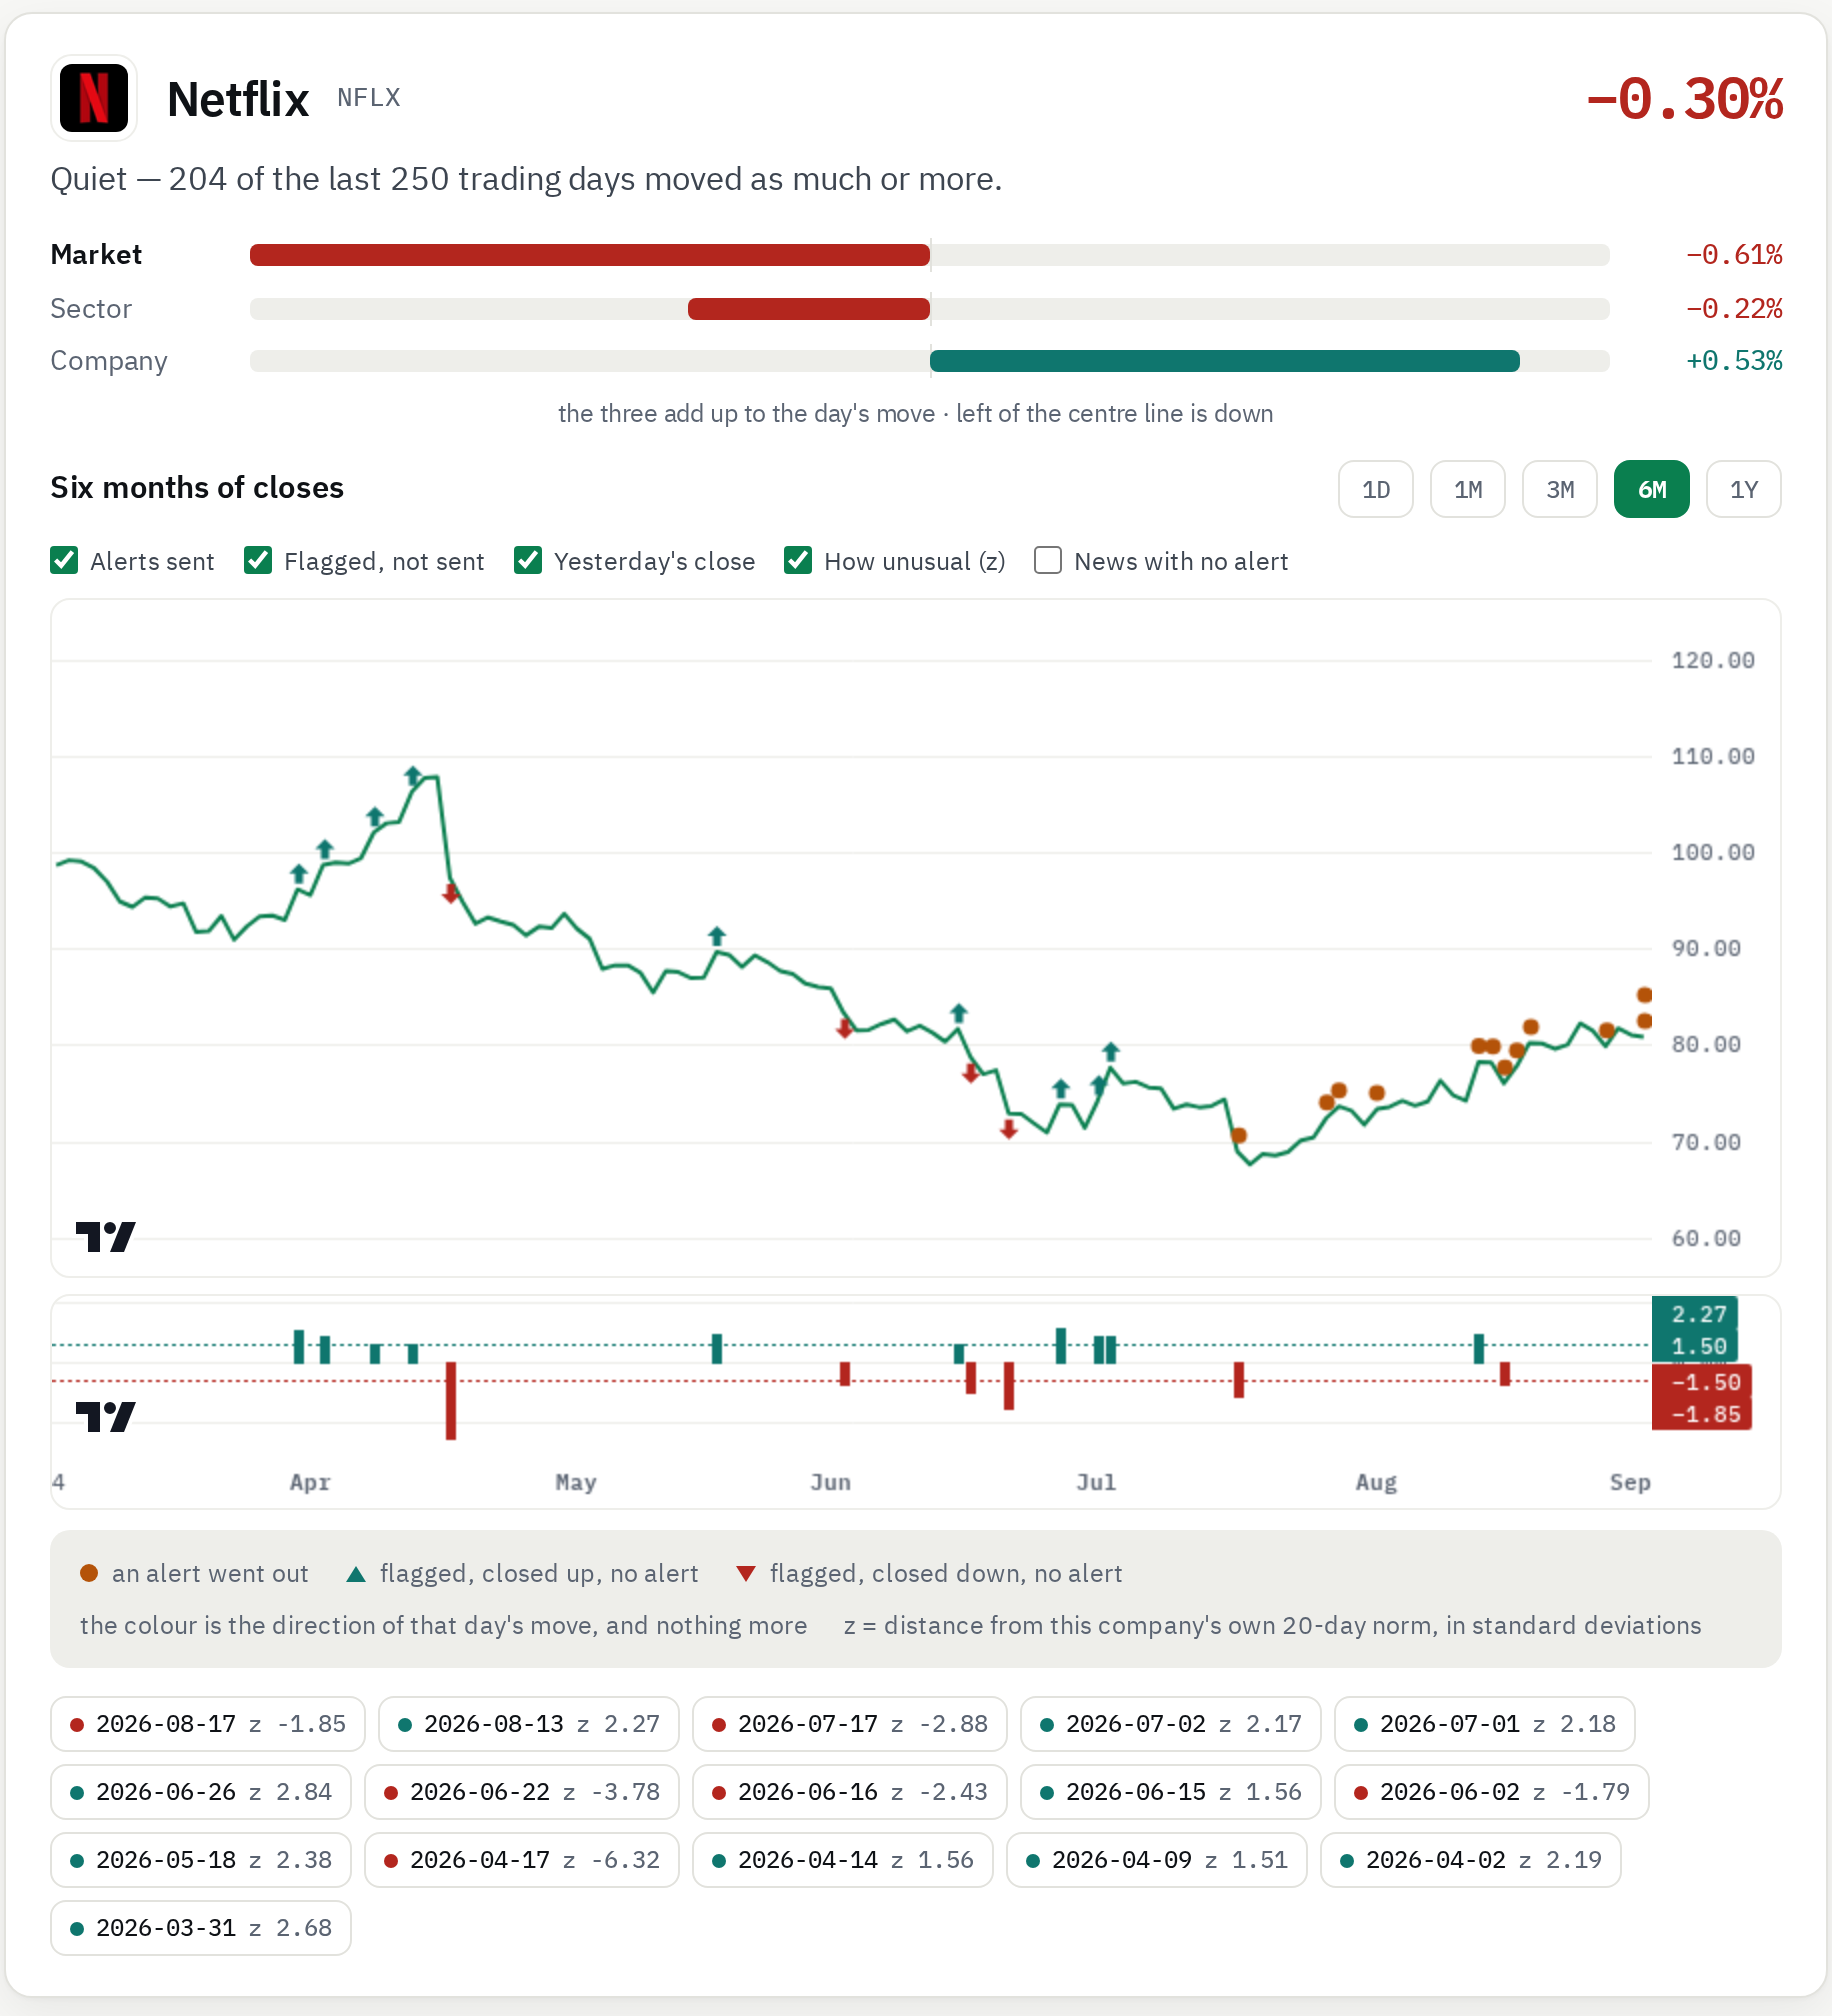
\includegraphics[height=0.68\textheight]{app_v7_empresa.png}
\end{column}
\begin{column}{0.35\textwidth}
\small
\textbf{1. É invulgar?}\\
{\footnotesize Em palavras, antes do número: $204$ dos últimos $250$ dias
moveram-se tanto ou mais. O veredicto é \emph{``Quiet''}, e é dito antes de qualquer valor.}
\vspace{3mm}

\textbf{2. Foi a empresa?}\\
{\footnotesize \textbf{Não.} A ação desce $0{,}30\%$, mas a contribuição da própria
empresa é \textbf{positiva} ($+0{,}53\%$): quem a puxa para baixo é o
\textbf{mercado} ($-0{,}61\%$). A percentagem sozinha mandava procurar na
empresa uma razão que estava fora dela.}
\vspace{3mm}

\textbf{3. Já aconteceu?}\\
{\footnotesize Os dias assinalados na curva, e os precedentes dentro do texto do alerta.}
\end{column}
\end{columns}
\end{frame}

% ══ 7. DEMONSTRAÇÃO ═════════════════════════════════════════════════════════
\begin{frame}{Demonstração}
\begin{center}
{\large O sistema está no ar.} \quad \textbf{[gravação]}\\[2mm]
{\footnotesize uma notícia real, do momento em que chega até ao alerta que sai}
\end{center}
\vspace{1mm}
\begin{center}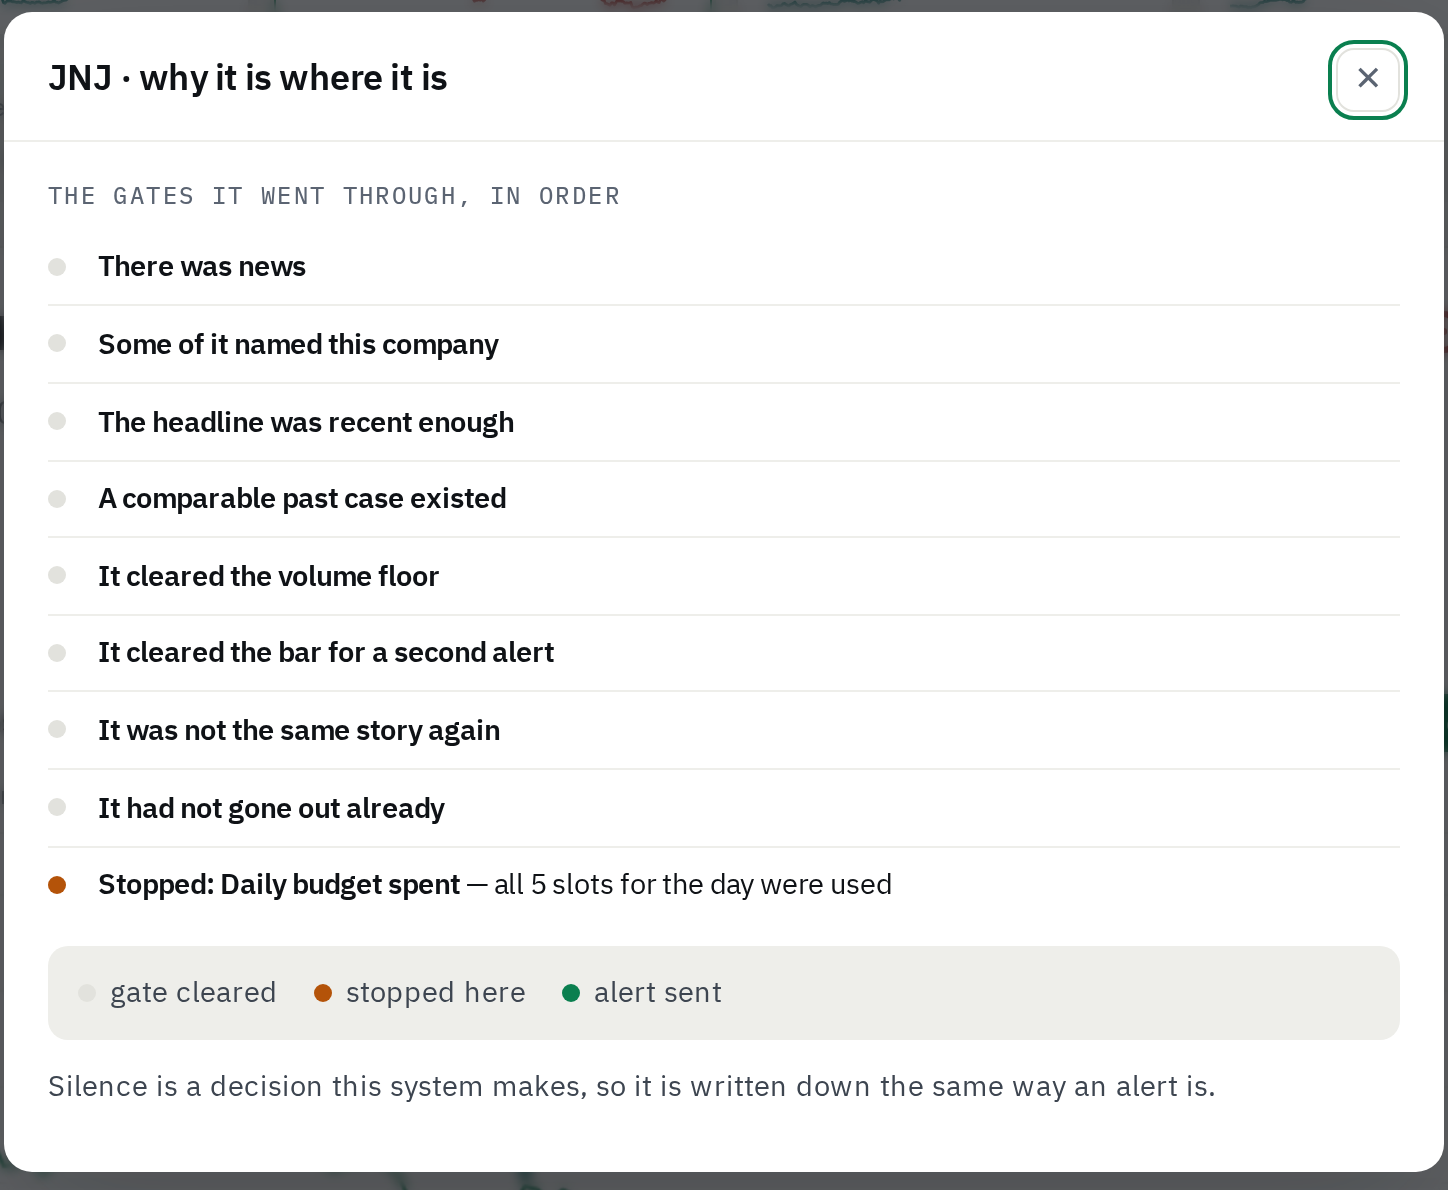
\includegraphics[width=0.97\textwidth,height=0.46\textheight,keepaspectratio]{app_v7_silencio.png}\end{center}

{\footnotesize O percurso de uma candidata pelas portas, até onde parou. \textbf{É a parte
que uma demonstração ao vivo não mostra}: nove em cada dez varreduras não enviam nada, e o
silêncio fica escrito como um alerta.}
% ⚠️ AO ALUNO: substituir a imagem acima pela GRAVAÇÃO no dia da defesa.
%    Opção A (mais segura): abrir o vídeo em janela separada e voltar aos slides.
%    Opção B: \usepackage{multimedia} e \movie[...]{...}{demo.mp4} — só funciona em
%             alguns leitores de PDF; testar no portátil da apresentação ANTES.
%    Plano B se não houver rede: esta imagem já mostra o essencial.
\end{frame}

% O que aprendi vive aqui, e nao num frame proprio: fica no ecra durante as perguntas,
% que e melhor sitio do que um slide que passa de relance.
\begin{frame}[plain]{O que aprendi}
\begin{enumerate}
  \item \textbf{A linha de base é tão importante como o modelo.}\\
        \footnotesize O resultado mais útil do trabalho veio de olhar para aquilo contra o qual eu
        estava a comparar.\\[2mm]
  \item \textbf{O sítio onde se põe um modelo importa tanto como o modelo.}\\
        \footnotesize O meu funcionava sozinho e deixou de servir atrás de dois filtros simples,
        que já faziam o trabalho.\\[2mm]
  \item \textbf{A técnica mais simples ganhou três vezes.}\\
        \footnotesize Ao Isolation Forest e ao modelo que lê o texto, que são \emph{simples contra
        complexo}. E uma tabela de constantes ganhou ao modelo implantado, que é um caso
        diferente: ali o modelo até era interpretável, e perdeu por \textbf{falta de informação}.
\end{enumerate}
\vspace{4mm}
\begin{center}
\small A parte difícil não foi escolher a técnica mais avançada.\\
Foi montar a avaliação \textbf{capaz de dizer que ela não era precisa}.\\[6mm]
{\Large \textbf{Obrigado.}\quad Perguntas?}
\end{center}
\end{frame}

\end{document}
